\documentclass[12pt,twoside]{article}

\usepackage{amsmath}
\usepackage{fancyhdr}
\usepackage{graphicx}
\usepackage{wrapfig}

\setlength{\oddsidemargin}{0pt}
\setlength{\evensidemargin}{0pt}
\setlength{\textwidth}{6.5in}
\setlength{\topmargin}{0in}
\setlength{\textheight}{8.5in}
\setlength{\headheight}{15pt}

\newcommand{\andrew}{Andrew Xia}
\newcommand{\psetnum}{6.115 Final Project Proposal}
\newcommand{\duedate}{Due: April $20^{\text{th}}$, 2016}
\renewcommand{\thesubsection}{\thesection.\alph{subsection}}

\pagestyle{fancy}
\fancyhead[L]{\andrew}
\fancyhead[C]{\psetnum}
\fancyhead[R]{\duedate}

\begin{document} 
\begin{center} {\bf \large \psetnum}
\\ \emph{3D Touchless Tracking Interface for Tic Tac Toe}
\\ {\bf \andrew}
\\ \duedate
\end{center}

\section{Introduction}
It's Spring 2016, and we're here with another spectacular 6.115 project proposal! For my final project, I hope to build a 3D touchless tracking interface and connect it with my 8051 and PSoC to allow users to play 3D tic tac toe with either each other or a computer AI. 
\\
\\ \emph{What interested you in the idea?} I am interested in this idea because I want to work on a project that has both an interesting and flashy hardware and software component. Writing the AI software for my 3D tic tac toe board will be a very rewarding and educational experience for me, and building the 3D tracing interface will also be very fun. 
\\ 
\\ \emph{Why is this project interesting?} This project is interesting because while 2D tic tac toe is a game familiar to all, 3D tic tac toe represents a game that while it is familiar, it can also be novel and entertaining. This project also uses a 3D touchless interface for user input, which is another novel way of interacting with software, as we are used to touching buttons or screens to communicate with devices in our daily lives. 
\\ Some ideas and features that I am thinking about including are:
\begin{itemize}
\item Build a 3D touchless tracking interface to effectively locate the user's hand position in three dimensions using large capacitive plates in the X, Y, and Z axes. 
\item Use VGA connection from the PSoC to display users profiles on a screen. 
\item Build a {\em capacitance based sensor} which will serve as the input module. Users can effectively ``swipe'' left or right based on my arrangement of the capacitance based sensors. 
\end{itemize}


\section{Hardware Description}
\begin{wrapfigure}{R}{0.3\textwidth}
\centering
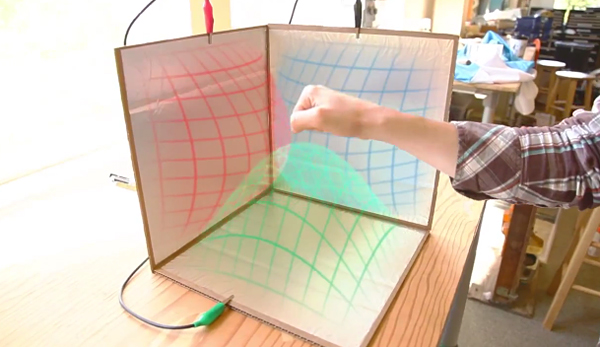
\includegraphics[width=0.25\textwidth]{3d_touch.jpg}
%\caption{\label{fig:frog1}test.}
\end{wrapfigure}
The key hardware component of my project will be building a 3D touchless interface, which is shown in the image to the side. The three aluminum foils (or a similar material) on the three sides are the capacitors that the human finger complements, and thie distance from each of the three capacitors will definite the capacitance of the capacitance, which we can measure using an ADC, and effectively pinpoint the 3D location of the human hand. 
\\ Another hardware interface I plan on creating is a normal capacitance based sensor. I can use AT42QT1010 chips which can create capacitive based sensors, which I can interface to create a swiping module. 
\\ I will use a 74LS245 chip to connect my PSoC to a VGA cable which can then display information on a screen. I will use what was covered in lecture to complete this task. 


\subsection{Hardware Schematic}
Below is a preliminary hardware schematic of my final project:
\begin{center}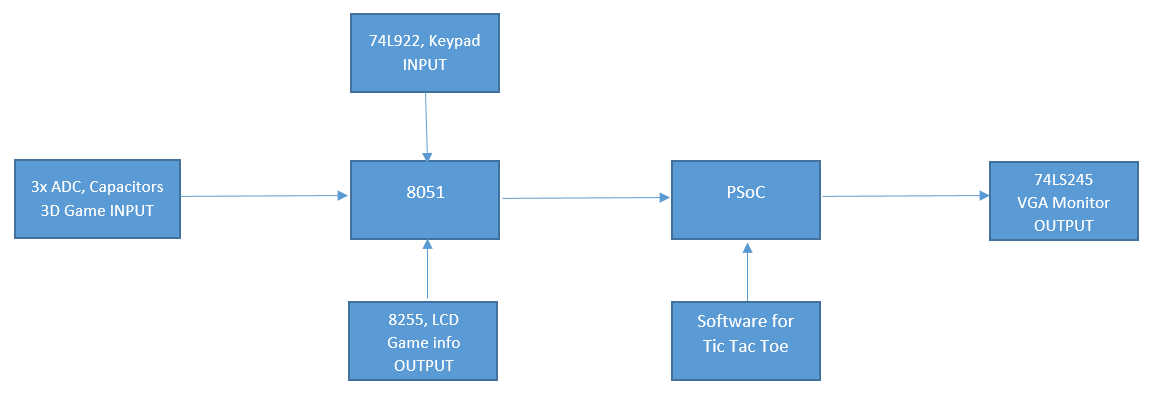
\includegraphics[width = 150mm]{Hardware_final.png} \end{center}

\section{Software Description}
As for my software, I will code my project in C, using the PSoC as my main control module, as it would would be more efficient to do so over writing code in assembly for the 8051. The Tic Tac Toe AI is not too software heavy, so I hope to develop the basic framework for my code and spend the rest of my extra time focusing on hardware improvements. 

\newpage
\subsection{Software Flowchart}
Below is a flowchart of my software: 
\begin{center}\fbox{\begin{minipage}{35em}

\begin{enumerate}
\item Initiate \& Reset Tic Tac Toe Board
\item Mode 1: two player Tic Tac Toe
	\begin{enumerate}
	\item User can view \& rotate, using 74L922 or capacitive-based sensors, current 3D tic tac toe board on VGA display
	\item User adds piece to the board by leaving hand in position of 3D touchless tracking interface for extended amound of time
	\item After entering piece on board, the other player can play. 
	\end{enumerate}
\item Mode 2: one player AI Tic Tac Toe
	\begin{enumerate}
	\item User can view \& rotate, using 74L922 or capacitive-based sensors, current 3D tic tac toe board on VGA display
	\item User adds piece to the board by leaving hand in position of 3D touchless tracking interface for extended amound of time
	\item After entering piece on board, computer plays against user and submits his move through AI algorithm. 
	\end{enumerate}
\item Reset the game and enter either mode through the 74C922 Keypad
\end{enumerate}

\end{minipage}} \end{center}


\section{Project Scope and Management}

\subsection{Modest risk level Project goals}
In this section, I discuss basic project goals that I believe I can meet. I expect myself to be able to build a functioning 3D touchless tracking interface without problem. I can confirm that the interface works by measuring 

\subsection{Adding the wow factor}
In this section, I discuss project goals that I plan on meeting. I would like to be able to display my 3D tic tac toe board on a monitor, using a VGA connection, in a very basic manner. 

\subsection{To make the project SPECTACULAR}
If I have extra time, I hope to write the AI for my 3D tic tac toe game. I would also like to make my visual display more user-friendly, adding rotate features and potentially animation to display a won game. 


\section{Special Component Needs}
\emph{What special chips will I need?} 
Chips I will use: 
\begin{enumerate}
\item ADC0804 to convert the analog capacitve based sensor signal to digital.
\item 8255, LCD to display basic user information
\item 74L922, 16-key keypad for resetting the Tic Tac Toe Game
\item 74LS245 to connect PSoC with VGA display
\end{enumerate}


\section{Timetable}
\begin{enumerate}
\item April 11 - 18
\\ \indent During this week, I thought harder about what project I want to work on for my 6.115 final project.
\item April 18 - 25
\\ \indent During this week, I want to finish making my 3D capacitance based sensor. I will make a initial version using cardboard to make sure that the sensors can function properly, and I will make a final, aesthetically more pleasing version.
\item April 25 - May 2
\\ \indent During this week, I hope to have a basic 3D tic tac toe software running. I can initially design a two player version of the game, in which two players will take alternating turns and make their respective moves. 
\item May 2 - 9
\\ \indent During this week, I hope to connect my VGA screen with the PSoC and microcontroller and be able to display my game in a visually pleasing way on a monitor. 
\item May 9 - 15
\\ \indent During this week, I can further improve the software or hardware aspects of my project, such as finishing building the AI for Tic Tac Toe or adding other hardware/software features to be determined. 
\end{enumerate}

\end{document}